%!TEX root=../document.tex

\section{Quantenkryptographie}
\label{sec:Quantenkryptographie}

\subsection{One-Time-Pad}

Das One-Time-Pad Verschlüsselungsverfahren funktioniert über einen geheimen Schlüssel welcher folgende Eigenschaften erfüllen muss: \cite{ontetimepadwiki}
\begin{itemize}
    \item er ist mindestens so lang wie die Nachricht
    \item er ist gleichverteilt zufällig gewählt
    \item er muss geheim bleiben
    \item er darf nicht wiederverwendet werden, auch nicht teilweise
\end{itemize}

Damit erfüllt ein One-Time-Pad Kerckhoffs’ Prinzip, welches besagt, dass die Sicherheit eines Kryptosystems nicht von der Geheimhaltung des Verschlüsselungsalgorithmus abhängen darf, sondern lediglich von der Geheimhaltung des Schlüssels.\cite{ontetimepadwiki}
Dies bedeudet, dass eine mit einem One-Time-Pad Verschlüsselte Nachricht auch mit beliebig hoher Rechenleistung nicht dechiffriert werden kann.

Beim One-Time-Pad handelt es sich also quasi um ein 'perfektes' Verschlüsselungssystem.
Das größte Problem des One-Time-Pads ist es allerdings, den geheimen Schlüssel an beide Parteien zu übertragen, ohne, dass dieser abgefangen wird.

\subsection{Quanten-Schlüsselaustausch}
\label{sec:Quanten-Schlusselaustausch}

Als Quantenschlüsselaustausch bezeichnet man Verfahren der Quanteninformatik, die Eigenschaften der Quantenmechanik nutzen, um zwei Parteien eine gemeinsame Zufallszahl zur Verfügung zu stellen.
Dies löst nun das größte Problem des One-Time-Pad, nämlich die sichere Übertragung des Schlüssels.

Der Quantenschlüsselaustausch funktioniert nach dem Prinzip, einen Angreifer (Man in the Middle) bei der Schlüsselgenerierung zu erkennen, da eine Messung eines Quantenmechanischen Zustandes, immer den Wert verändert.

\subsubsection{Funktionsweise}

Die Informationen werden mittels Photonen übertragen. Photonen können horizontal oder vertikal polarisiert sein (– oder |). Ein horizontal polarisiertes Photon wird von einem vertikalen Filter reflektiert, durch einen horizontalen durchgelassen.
Außerdem können Photonen verschiedenartig diagonal polarisiert sein (/, “rechtsdiagonal“, oder \textbackslash, “linksdiagonal“). Diese werden wieder von ihren respektiven Filtern reflektiert, oder durchgelassen.
Daraus ergeben sich nun 2 Basen, die +-Basis (- und |) und die $\times$-Basis (/ und \textbackslash).
Jede Polarisation einer Basis bekommt nun einen anderen binären Wert zugewiesen, wobei die Wahl dabei irrelevant ist, sie muss nur bei beiden Parteien gleich sein. 

\begin{figure}[!htb]
	\centering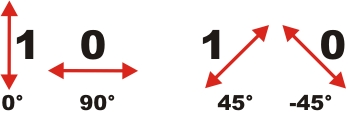
\includegraphics[width=0.6\textwidth]{images/polarisation}
	\caption{Messbasis + (links) und Messbasis $\times$ (rechts) \cite{quantenschluesselaustausch}}
	\label{fig:polarisation}
\end{figure}

Nun beginnt der Sender der Nachricht (Alice) an, einzelne Photonen an den Empfänger (Bob) zu verschicken. Beide Wählen dabei komplett zufällig, mit gleich großer Wahrscheinlichkeit eine Basis aus. 
Alice wählt nun weiters, wieder komplett zufällig und mit gleich großer Wahrscheinlichkeit eine Polarisation und sendet ein Photon an Bob.

Wenn Bob nun zufällig die gleiche Basis wie Alice verwendet hat, bekommt dieser ein gültiges Ergebnis (also 0 oder 1), wenn er allerdings eine andere basis verwendet hat wird das gesendete Photon zu 50\% reflektiert oder durchgelassen, ergibt also zu 50\% 0 oder 1, diese Messung ist nicht brauchbar und wird später verworfen.

Nachdem Alice genügend Photonen an Bob geschickt hat, müssen beide Parteien noch bestimmen, welche Messwerte für den Schlüssel verwendet werden sollen.
Dafür machen Alice und Bob die Wahl ihrer Messbasis öffentlich, jedoch nicht welche Polarisation gesendet bzw. empfangen wurde. Sie veröffentlichen also beide eine Liste mit denen von ihnen gewählten Basen (+ oder $\times$).
Schlussendlich vergleichen beide nun diese Listen, wenn sie bei einer Übertragung die gleiche Basis verwendet haben wird der Wert für den Schlüssel verwendet, ansonsten einfach verworfen.
Dadurch also werden also ungefähr 50\% der gesendeten Bits für die Schlüsselgenerierung verwendet.

\begin{table}[!htb]
    \parbox{.45\linewidth}{
        \centering
        \begin{tabular}{|c|c|c|}
        \hline
        Photon      & Basis             & Bit           \\ \hline
        \textbf{1}  & \textbf{+}        & \textbf{1}    \\ \hline
        2           & $\times$          & 1             \\ \hline 
        \textbf{3}  & \textbf{+}        & \textbf{0}    \\ \hline
        4           & +                 & 1             \\ \hline
        \textbf{5}  & \textbf{$\times$} & \textbf{1}    \\ \hline
        \textbf{6}  & \textbf{+}        & \textbf{0}    \\ \hline
        \textbf{7}  & \textbf{$\times$} & \textbf{0}    \\ \hline
        8           & $\times$          & 1             \\ \hline
        \end{tabular}
        \caption{Beispielübertragung Alice}    
    }

    %\parbox{.45\linewidth}{
    %    \centering
    %    \begin{tabular}{|c|c|c|}
    %    \hline
    %    Photon      & Basis             & Bit           \\ \hline
    %    \textbf{1}  & \textbf{+}        & \textbf{1}    \\ \hline
    %    2           & +                 & 0             \\ \hline 
    %    \textbf{3}  & \textbf{+}        & \textbf{0}    \\ \hline
    %    4           & $\times$          & 1             \\ \hline
    %    \textbf{5}  & \textbf{$\times$} & \textbf{1}    \\ \hline
    %    \textbf{6}  & \textbf{+}        & \textbf{0}    \\ \hline
    %    \textbf{7}  & \textbf{$\times$} & \textbf{0}    \\ \hline
    %    8           & +                 & 0             \\ \hline
    %    \end{tabular}
    %    \caption{Beispielübertragung Bob}
    %}
    
    \label{table:alice-bob-uebertragung}
\end{table}
    
In diesem Beispiel sind die \textbf{Fett} hervorgehoben Basen gleich, also wäre der generiert Schlüssel von Alice und Bob 10100; jeweils Photon 1, 3, 5, 6, 7 werden verwendet, die anderen verworfen.

\subsubsection{Abhörsicherheit}

Bei dem obigen Verfahren ist es nun auch möglich Abhöhrsicherheit zu garantieren, sodass eine dritte Person (Eve) sich nich zwischen die Kommunikation schalten und den Schlüsselaustausch abfangen kann.
Um die Kommunikation abzufangen kann Eve sich nun zwischen Bob und Alice schalten und auch rein zufällig eine Basis wählen und das Photon messen.
Eve muss allerdings sofort wieder ein neues Photon an Bob senden, in 50\% der Fälle wählt Eve zur Messung jedoch die falsche Basis und sendet dadurch ein falsches bit an Bob.
Diesen durch Eve verursachten Fehler können Alice und Bob nun bemerken, wenn Alice und Bob die gleiche Basis gewählt haben, sie bei gleicher Wahl der Basis immer eindeutige Ergebnisse erhalten sollten.

\begin{table}[ht]
    \centering
    \begin{tabular}{|c|c|c|c|c|}
    \hline
    Basis Alice/Bob     & Basis Eve & Empfang Bob   & Übereinstimmung Alice und Bob \\ \hline
    +~+                 & +         & Eindeutig     & 100\% \\ \hline
    +~+                 & $\times$  & Zufall        & 50\%  \\ \hline 
    $\times$~$\times$   & +         & Eindeutig     & 50\%  \\ \hline
    $\times$~$\times$   & $\times$  & Zufall        & 100\% \\ \hline
    
    \end{tabular}
    \caption{Möglichkeiten der Übertragung mit Eve als Man-in-the-Middle \cite{quantenschluesselaustausch}}
    \label{table:eve-moeglichkeiten}
\end{table}

Insgesamt gibt es allerdings, wenn Alice und Bob die gleiche Basis gewählt haben in 25\% der Fällen falsche Messergebnisse. 
Um Eve also zu entdecken müssen Bob und Alice nach der Erfolgreichen Übertragung einen Abgleich von einigen (nicht allen!) Werten, bei denen sie die gleiche Basis verwendet haben durchführen, gibt es dort über 25\% Diskrepanz zwischen den Werten, ist sehr Wahrscheinlich ein Man-in-the-Middle Angriff durchgeführt worden.
In diesem Fall muss der generiert Schlüssel verworfen und anders eine neuer Verbindung hergestellt werden. 


\subsection{Post-Quantum-Kryptographie}
\label{sec:Post-Quantum-Kryptographie}

Ein besonderer Teil der Quantenkryptographie stellt die Post-Quantum-Kryptographie dar.
Diese behandelt sich mit der Tatsache, dass alle modernen asymmetrischen Verschlüsselungsverfahren durch die Entwicklung eines Quantencomputers unbrauchbar werden (siehe \ref{sec:Shor's Algorithmus} Shor's Algorithmus).
Damit also momentane Kommunikation auch in Zukunft nicht entschlüsselt werden kann, benötigt man auch jetzt schon Verschlüsselungsverfahren, welche auch Quantencomputer in Zukunft nicht knacken können. \cite{postquantumwiki}


\section{Quantenalgorithmik}
\label{sec:Quantenalgorithmik}


\subsection{Besonderheiten und Unterschiede zu 'klassischer' Algorithmik}
\label{sec:Besonderheiten und Unterschiede zu klassischer Algorithmik}


\subsection{Quantenalgorithmik Übersicht}
\label{sec:Quantenalgorithmik Übersicht}


\subsubsection{Deutsch-Josza Algorithmus}

Dieser Algorithmus kann zu Lösen sogenannter Blackbox-Probleme verwendet werden, für die normale Computer exponentiell viele Zugriffe, ein Quantencomputer allerdings nur einen bräuchte.
Hierbei wird z.B. das Ergebnis einer Funktion \textit{f} darauf überprüft, ob alle Eingaben konstant 0 als Ergebnis liefern, oder ob nur die Hälfte 0 und die andere Hälfte 1 liefert. \cite{quantenalgorithmgwiki}


\subsubsection{Simons's Algorithmus}

Dieser Algorithmus dient auch zur exponentiell schnelleren Lösung von Blackbox-Problemen und war Vorbild für Shor's Algorithmus. \cite{quantenalgorithmgwiki}

\subsubsection{Quanten Phasen Näherungs-Algorithmus}

\begin{quote}
    \textit{The quantum phase estimation algorithm is used to determine the eigenphase of an eigenvector of a unitary gate given a quantum state proportional to the eigenvector and access to the gate.}\cite{quantenalgorithmgwiki}
\end{quote}
Der Algorithmus wird außerdem oft als Unterfunktion in anderen Algorithmen verwendet. 

\subsection{Shor's Algorithmus}
\label{sec:Shor's Algorithmus}



